%!TEX root = ../Report.tex

In this chapter we summarise the implementation of the system produced last year, to get an idea of how a complete contention aware plastic parallel programming library could be produced. We then go on to cover the implementation details of the synthetic test program produced for this year of the project. Finally, we note a parallel programming pitfall that we encountered, which provides some insight as to why parallel programming is a challenge.



\section{Last Year's Implementation}
\label{section:implementation:last_years_implementation}

In this section, we give an overview of the implementation of the system produced last year. The purpose of this is to get a feel of how a contention aware plastic parallel programming library could be implemented, to provide context for this year's investigation.

We start with our implementation of a basic parallel skeleton, then we cover adding plasticity, and contention aware scheduling. C++ was used for speed, and the parallel backend used was Pthreads due to its wide availability, and fine level of control. 



\subsection{Skeleton Foundation}
\label{section:implementation:skeleton_foundation}

The skeleton we chose to implement was a map-array skeleton, as the map-array pattern is a widely used pattern with lots of applications. It consists of the common map pattern, where a given operation is applied to all elements of a sequence, with the addition of providing the operation with an additional array of supplementary data which can be accessed at any time.

This was done in C++ using a templated function which takes another function (supplied by the user) as an argument. The interface of this skeleton is given in figure \ref{fig:implementation_map_array_interface}, and a usage example in figure \ref{fig:implementation_map_array_usage_example}. These figures have been taken from the work done in the previous year \cite{me}.



\begin{figure}[H]
	\begin{lstlisting}

	template <typename in1, typename in2, typename out>
	void map_array(deque<in1>& input1, 
				   	deque<in2>& input2, 
				   	out (*user_function) (in1, deque<in2>), 
				   	deque<out>& output, 
				   	string output_filename = "", 
				   	parameters params = parameters())

	\end{lstlisting}

	\caption{Interface of the map\_array skeleton. The first four variables are the two input arrays, the function to apply, and the output array respectively. The output\_filename variable is the filename to record the metrics output in, and params sets up the initial parameters we will use. These last two are optional. This figure has been taken from the report of the previous year.}
	\label{fig:implementation_map_array_interface}
\end{figure}



\begin{figure}[H]
	\begin{lstlisting}
	int user_function(int in1, deque<int> in2) {
		return in1 + in2[in1];
	}

	int main() {
		// Inputs.
		deque<int> input1(ARRAY_SIZE);
		deque<int> input2(ARRAY_SIZE_2);

		// Put data in inputs.

		// Output.
		deque<int> output(ARRAY_SIZE);

		// Start mapArray.
		map_array(input1, input2, user_function, output);

		// Record output.
	}
	\end{lstlisting}

	\caption{A usage example of map\_array, here we apply our user\_function to each element of input1. The size of our two input arrays need not match, but the size of the input1 and output arrays must. This figure has been taken from the report of the previous year.}
	\label{fig:implementation_map_array_usage_example}
\end{figure}



\subsection{Adding Plasticity}
\label{section:implementation:adding_plasticity}
To make this skeleton plastic at runtime, we stop all computation, terminate worker threads, update the parameters, and spawn new worker threads. To facilitate this, we utilised a bag of tasks, to allow for tasks to be put back into the bag, amongst other conveniences including providing common semaphores for inter-thread communication.


\subsection{Contention Aware Scheduling}
\label{section:implementation:contention_aware_scheduling}

In order for all the programs to synchronise and agree upon the parameters to use, we use a separate controller application, from which each program receives its parameters, and subsequent updates. To achieve this, along with a separate controller program, we reuse the original thread which spawns the worker threads to communicate with the main controller and update parameters when necessary. This system is illustrated at a high level in figure \ref{fig:controller_flowchart}, which expands upon figure \ref{fig:communication_structure}. These figures have been taken from the work done in the previous year \cite{me}.



\begin{figure}[H]
	\centering
	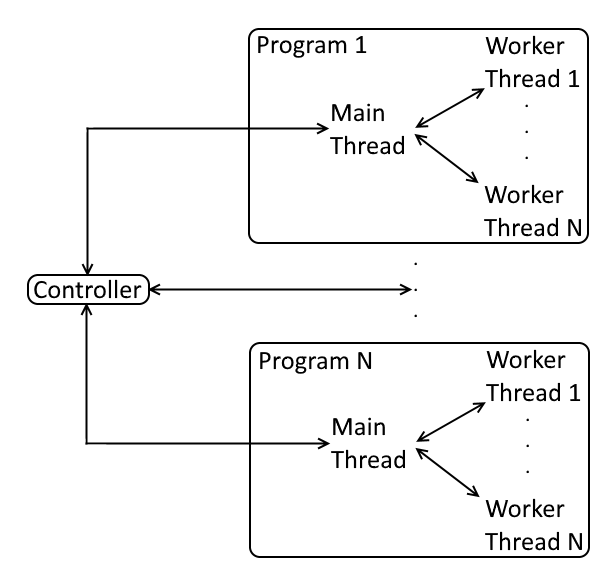
\includegraphics[width=\textwidth]{graphics/communication_structure.png}
	\caption{High level communication model of the system, with an arbitrary number of programs, with an arbitrary number of threads. Two way communication occurs between the controller and each main thread, and then between each main thread and its worker threads. This figure has been taken from the report of the previous year.}
	\label{fig:communication_structure}
\end{figure}



\begin{figure}[H]
	\centering
	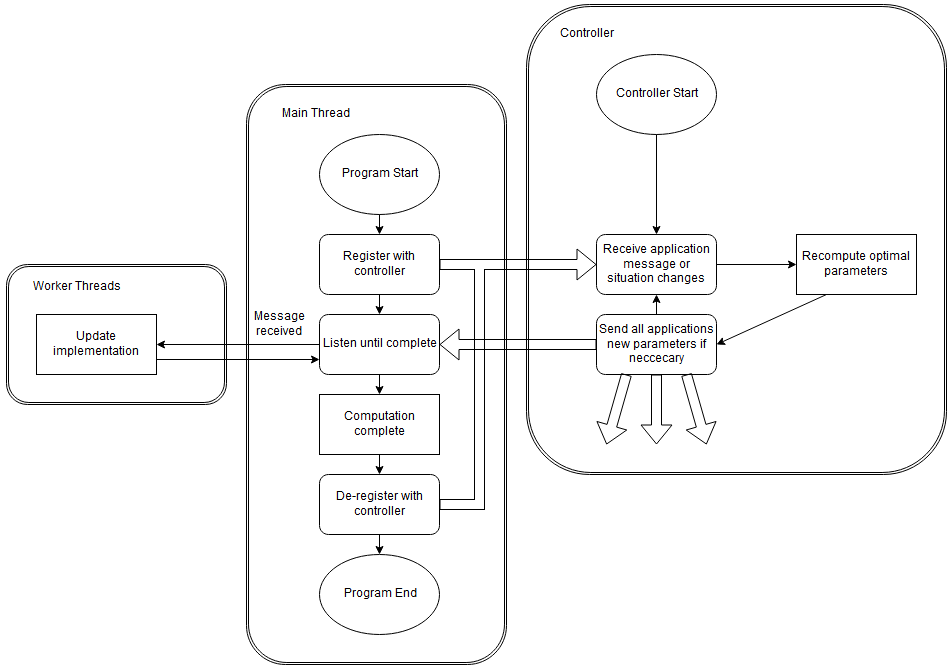
\includegraphics[width=1.1\textwidth]{graphics/controller_communication_flowchart.png}
	\caption{Communication model for communications between applications and the controller. Thin lines represent program flow, thick lines represent inter-process messages. This figure has been taken from the report of the previous year.}
	\label{fig:controller_flowchart}
\end{figure}



When this switching is done and what the new parameters should be is another matter. In this project, we demonstrate how a contention aware plastic parallel programming system might be implemented, that the overhead incurred is acceptable, and we show the potential performance gains. A complete system would calculate when to switch parameters and what they would be, based upon the current state of the machine. However, for last year's investigation, we manually control these things in a synthetic environment, and communicate them to the main thread using the controller application, as this was adequate for our investigation.



\section{Implementation of the Synthetic Test Program}
\label{section:implementation:implementation_of_the_synthetic_test_program}

In this section we cover the implementation details of the system we produced this year. The main focus is our synthetic test program, which is designed to perform a test of a stencil code, with given parameters and for a given number of repeats. It does not handle changing parameters for different tests, this is left to our experiment scripts. In the next chapter, chapter \ref{chapter:experimental_methodology}, we give details of other software that we produced, as well as modifications made to our synthetic test program in the context of specific experiments.



\subsection{High Level Plan}
\label{section:implementation:high_level_plan}

In contrast to the contention aware plastic parallel programming library that we built last year, this year we do not require a controller application. This is because we are not interested in the overhead incurred with the implementation, but rather with assessing the possible gains that could be had, and overall if a contention aware plastic parallel programming library would be valuable.

This changes our focus, meaning that there will be less work to be done on communication and synchronisation, but more care needs to be taken with regards to parallel performance and producing a suitable synthetic stencil workload, particularly with this more complex parallel pattern.

We intend our synthetic test program to be a part of a larger experimental framework. The outline of how this should operate is as follows: 

A complete experiment consists of multiple tests of our synthetic test program with varying parameters. Accordingly, we utilise an experiment script, written in bash, which will handle changing the parameters for each test, and niceties such as reporting the progress of the experiment. It will compile and run our synthetic test program, supplying it with appropriate parameters. The synthetic test program will save its output in an appropriate directory, ready for later analysis with a data analysis program tailored to the current experiment. 

Our synthetic test program will have two distinct phases, a setup phase and a processing phase. The high level plan for how our synthetic test program should operate is as follows:



\subsubsection{Setup Phase}
\label{section:implementation:setup_phase}

\begin{itemize}
    \item Read configuration and set appropriate parameters
    \item Initialise the data grid with given size
    \item Calculate row allocations to divide said grid between the given number of threads
    \item Setup data structures for additional features, such arrays for the convergence test, and semaphores for barrier synchronisation (These features are discussed in section \ref{section:design:performance_characteristics_investigation}.)
\end{itemize}



\subsubsection{Processing Phase}
\label{section:implementation:procesing_phase}

\begin{itemize}
    \item Setup timekeeping functions
    \item Spawn worker threads
    \item Perform computation of the stencil code, recording the time taken
    \item Format and save output data for later analysis
\end{itemize}



\subsection{Implementation}
\label{section:implementation:implementation}

In this section we give the specifics of the implementation of our synthetic test program. We start by describing some general features of the program, then we break it down into the setup phase and the processing phase, as described in the high level plan, in section \ref{section:implementation:high_level_plan}.

The synthetic test program is implemented in C++. We chose C++ for its speed, and advanced language features such as templates. The parallel code was implemented using the C++ std::threads library, which provides an improved interface using pthreads as its back end.

Many aspects of the program are tuned for performance, such as minimising function calls the use of appropriate data structures. Also in the name of performance, and of correctness, for features which are switched on and off between tests in an experiment, (such as barrier synchronisation,) we use the C++ preprocessor to include or remove the actual code at compile time, according to compiler flags. This is so that, if a feature is switched off, its code is not even included in the binary file, meaning it has no effect on our performance. An example of how this is done can be found in appendix \ref{appendix:code_snippets}, which shows the preprocessor commands and how they switch features in our worker function.

Another consideration which can affect our performance is a cold CPU cache. The CPU cache is a structure which stores data for faster lookup, and is particularly relevant to multiprogramming workloads, as we may encounter synchronisation issues \cite{agarwal_hennessy_horowitz_1988}. However, When we first start our program, the cache will be cold, as it contains no useful data. So our first run by our synthetic test program will be affected by the cold cache, as it loads data into the cache. Subsequent runs would not be affected, as the cache would have ``warmed up''. To combat this, we perform one extra run at the start of our computation, and we disregard its execution time when we are analysing the data from the experiment.



\subsubsection{Setup Phase}
\label{section:implementation:setup_phase2}

The first thing to be done by our synthetic test program is to read the configuration given. This is provided as a set of parameters in a text file, which control each aspect of the test. In short, these aspects are: the number of repeats, the size of the data grid, the number of iterations (passes) over said grid, the computation to perform at each point, the number of workers to use and which virtual CPU core(s) they should use. This covers the features we described in section \ref{section:design:performance_characteristics_investigation}. The exact details of the configuration file are given in section \ref{section:experimental_methodology:experiment_infrastructure}.

Reading this configuration file was done using a custom implementation, rather than utilising an existing library, for precise control over the configuration file format.

Next, we initialise the data grid, which uses double precision floating point values, as this is a common format in scientific computing. So much so that work has been done to facilitate its use for scientific computing \cite{floating_point_example}.

Along with the data grid, we must initialise additional grids for the worker threads to store intermediate values between iterations. Two arrays are used, one to store the values from the previous iteration, and one to contain newly computed values. After an iteration, the roles of these arrays are reversed. This technique of using two arrays, named double buffering, is done to minimise the necessary synchronisation overhead, and is a common technique in performance conscious applications \cite{deng_wang_yan_yang_2008, sheeparamatti_sheeparamatti_bharamagoudar_ambali_2006}.

In the final part of the setup phase, we divide the data grid to allocate between the given number of threads, and setup our other data structures.



\subsubsection{Processing Phase}
\label{section:implementation:processing_phase2}

At the start of the processing phase, we record the current time. We go on to start the given number of worker threads, which will perform the main computation (the code for these worker threads can be seen in appendix \ref{appendix:code_snippets}.)

The worker threads then iterate over the grid, performing the basic jacobi computation at each point (that is, compute and record the mean of the points neighbours.) However, we wish to add an additional computation at each point, one that we can control, which can stress different resources and perform a set amount of work. This workload must be predictable (for repeatability,) scalable (for varying performance characteristics,) and efficient with regards to parallelism (for validity.) This is the main section of the processing phase, and is an important part of our synthetic test program. The rest of this section is dedicated to how we went about creating these workloads.

We want a set of workloads with different performance characteristics, which stress different components. As discussed in \ref{section:design:interesting_instances}, this should make for valuable test cases. Accordingly, we start with workloads which stress different aspects of a system. These include the CPU, virtual memory, hard disk, and low-level I/O. We chose to focus on the most common performance critical resources, the CPU and the memory. We looked at existing parallel performance tests to inform our decisions \cite{hackenberg_ilsche_schone_molka_schmidt_nagel_2013, stress}.

Again, as discussed in section \ref{section:design:interesting_instances}, we target two scenarios for each synthetic stencil workload. One with a small amount of work, meaning the overhead will be more significant, so more threads may not necessarily be a good thing, and one with a large amount of work, which can always use more threads than we have. We can do this simply by changing the grid size, but for more fine grained control, we also wish to vary the complexity of the calculations performed at each point in the grid.

To achieve this, all of our synthetic stencil workloads consist of some sort of work, contained in a loop. This loop serves two purposes, it beefs up our workload functions such that they can have a significant effect on runtime, and they provide linear control over the weight of our workload, allowing us to vary it for different experiments.

For example, one of our final workloads designed to stress the CPU consisted of a loop performing one square root operation, using the loop iterator as input. The square root function was used as it is a commonly used, reasonably expensive operation. This is the workload we use to describe the issues we had with compiler optimisation in the next section.



\section{A Parallel Programming Pitfall}
\label{section:implementation:a_parallel_programming_pitfall}

In this section, we present an aside describing a problem encountered during the development of the software required for this project. It illustrates the challenges of parallel programming. 

Our workload is synthetic with no actual effect. As such, it is vulnerable to compiler optimisation. Since we are carrying out performance critical experiments, we compile our application at GCC optimisation level 3, which can be quite smart in removing redundant loops amongst other optimisations. Our workload entirely consists of redundant loops, and so was consistently optimised away, as shown in figure \ref{fig:compiler_explorer_example}. As it transpires, this can be a particularly tricky problem to overcome.



\begin{sidewaysfigure}[hp]
    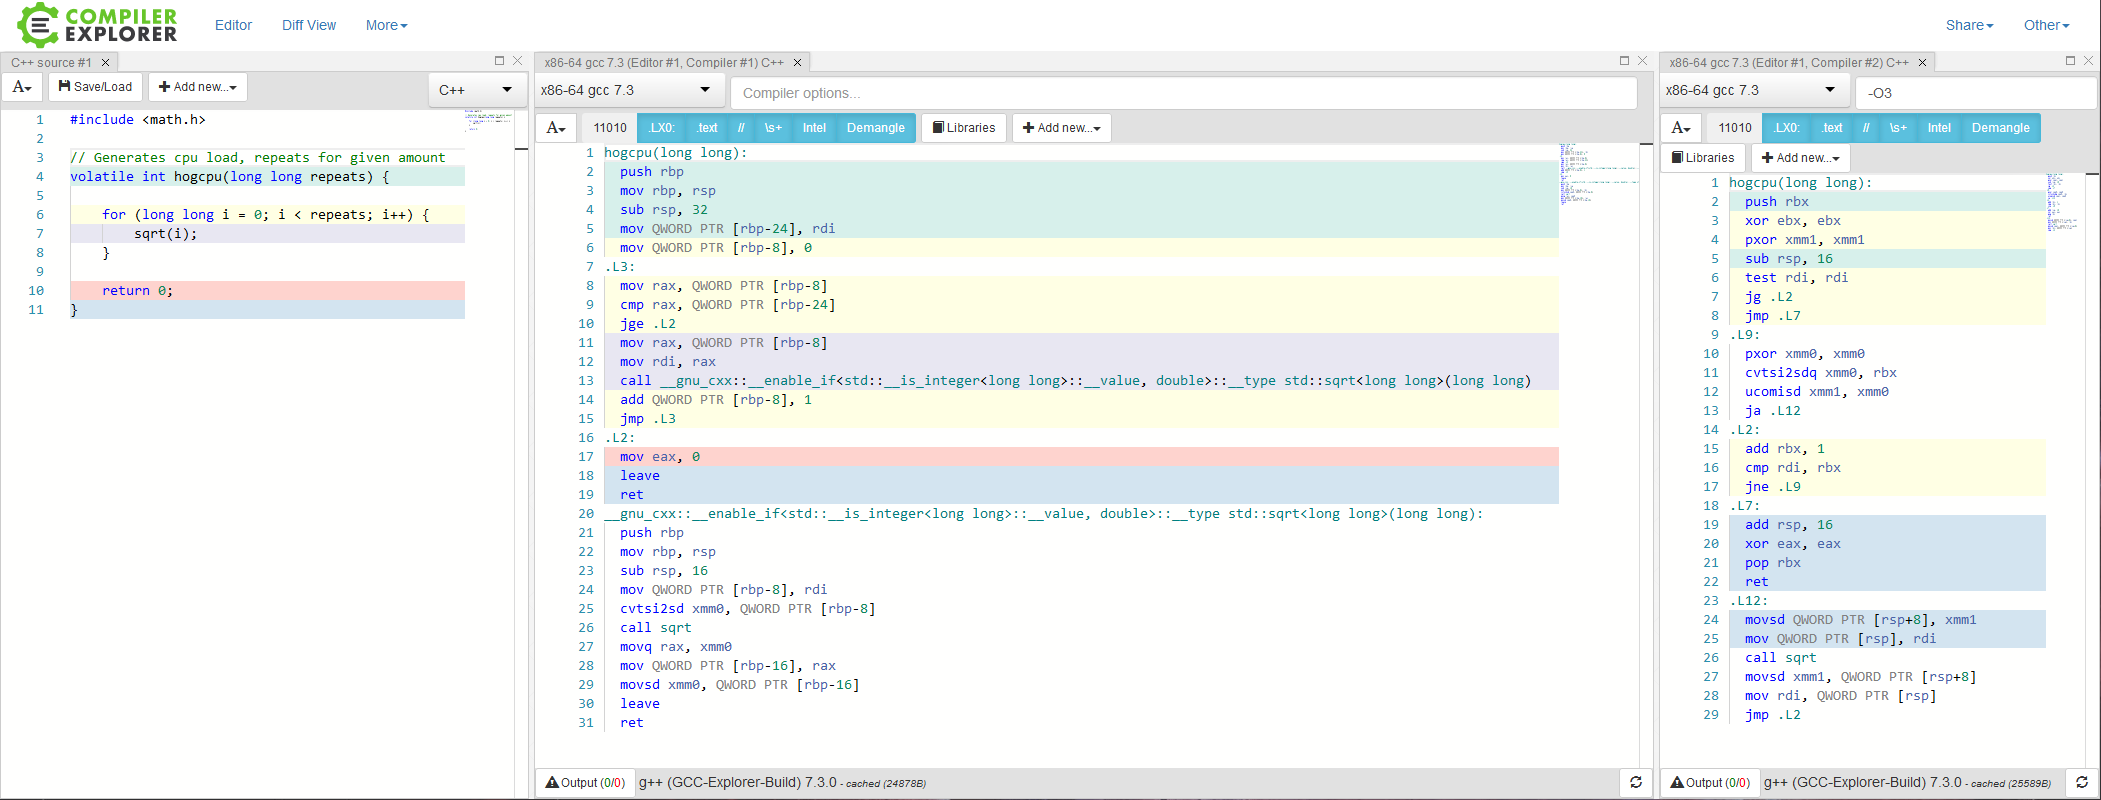
\includegraphics[width=\textwidth]{graphics/compiler_explorer_example.png}
    \caption{This figure shows that our workload function (sqrt()) is optimised away at optimisation level 3. Note - Colour coded regions show where the C++ code matches the machine code. \\
            Left: Original C++ code, Middle: Machine code produced by GCC at optimisation level 0, Right: Machine code produced by GCC at optimisation level 3 \\
            This tool \cite{compiler_explorer} proved to be useful during diagnosis of this problem.}
    \label{fig:compiler_explorer_example}
\end{sidewaysfigure}



The first attempt at a fix was to vary the input to sqrt function. If done in an unpredictable way, the compiler wouldn't be able to optimise our workload away. To do this, we thought of storing a random sequence of numbers, and iterating over this to provide input for sqrt. However, this would introduce more memory reads, slowing our computation and corrupting our workload from a purely CPU dependant workload. Also, the compiler may have still optimised away our workload, since we are using precomputed inputs, and we do nothing with the resulting value.

Our second idea was to generate random numbers to use as input to the workload. Moving the random number generation into the workload lets us circumvent any memory use. We can use rand() with a constant seed, since we are not concerned with true randomness, and we want repeatable results.

In validating this, we found that the workload was not being optimised out, and that we could vary the workload and the time taken would vary accordingly. However, with a more detailed analysis, we came across some confusing results, presented in figure \ref{fig:optimal_threads_1}.



\begin{figure}[H]
    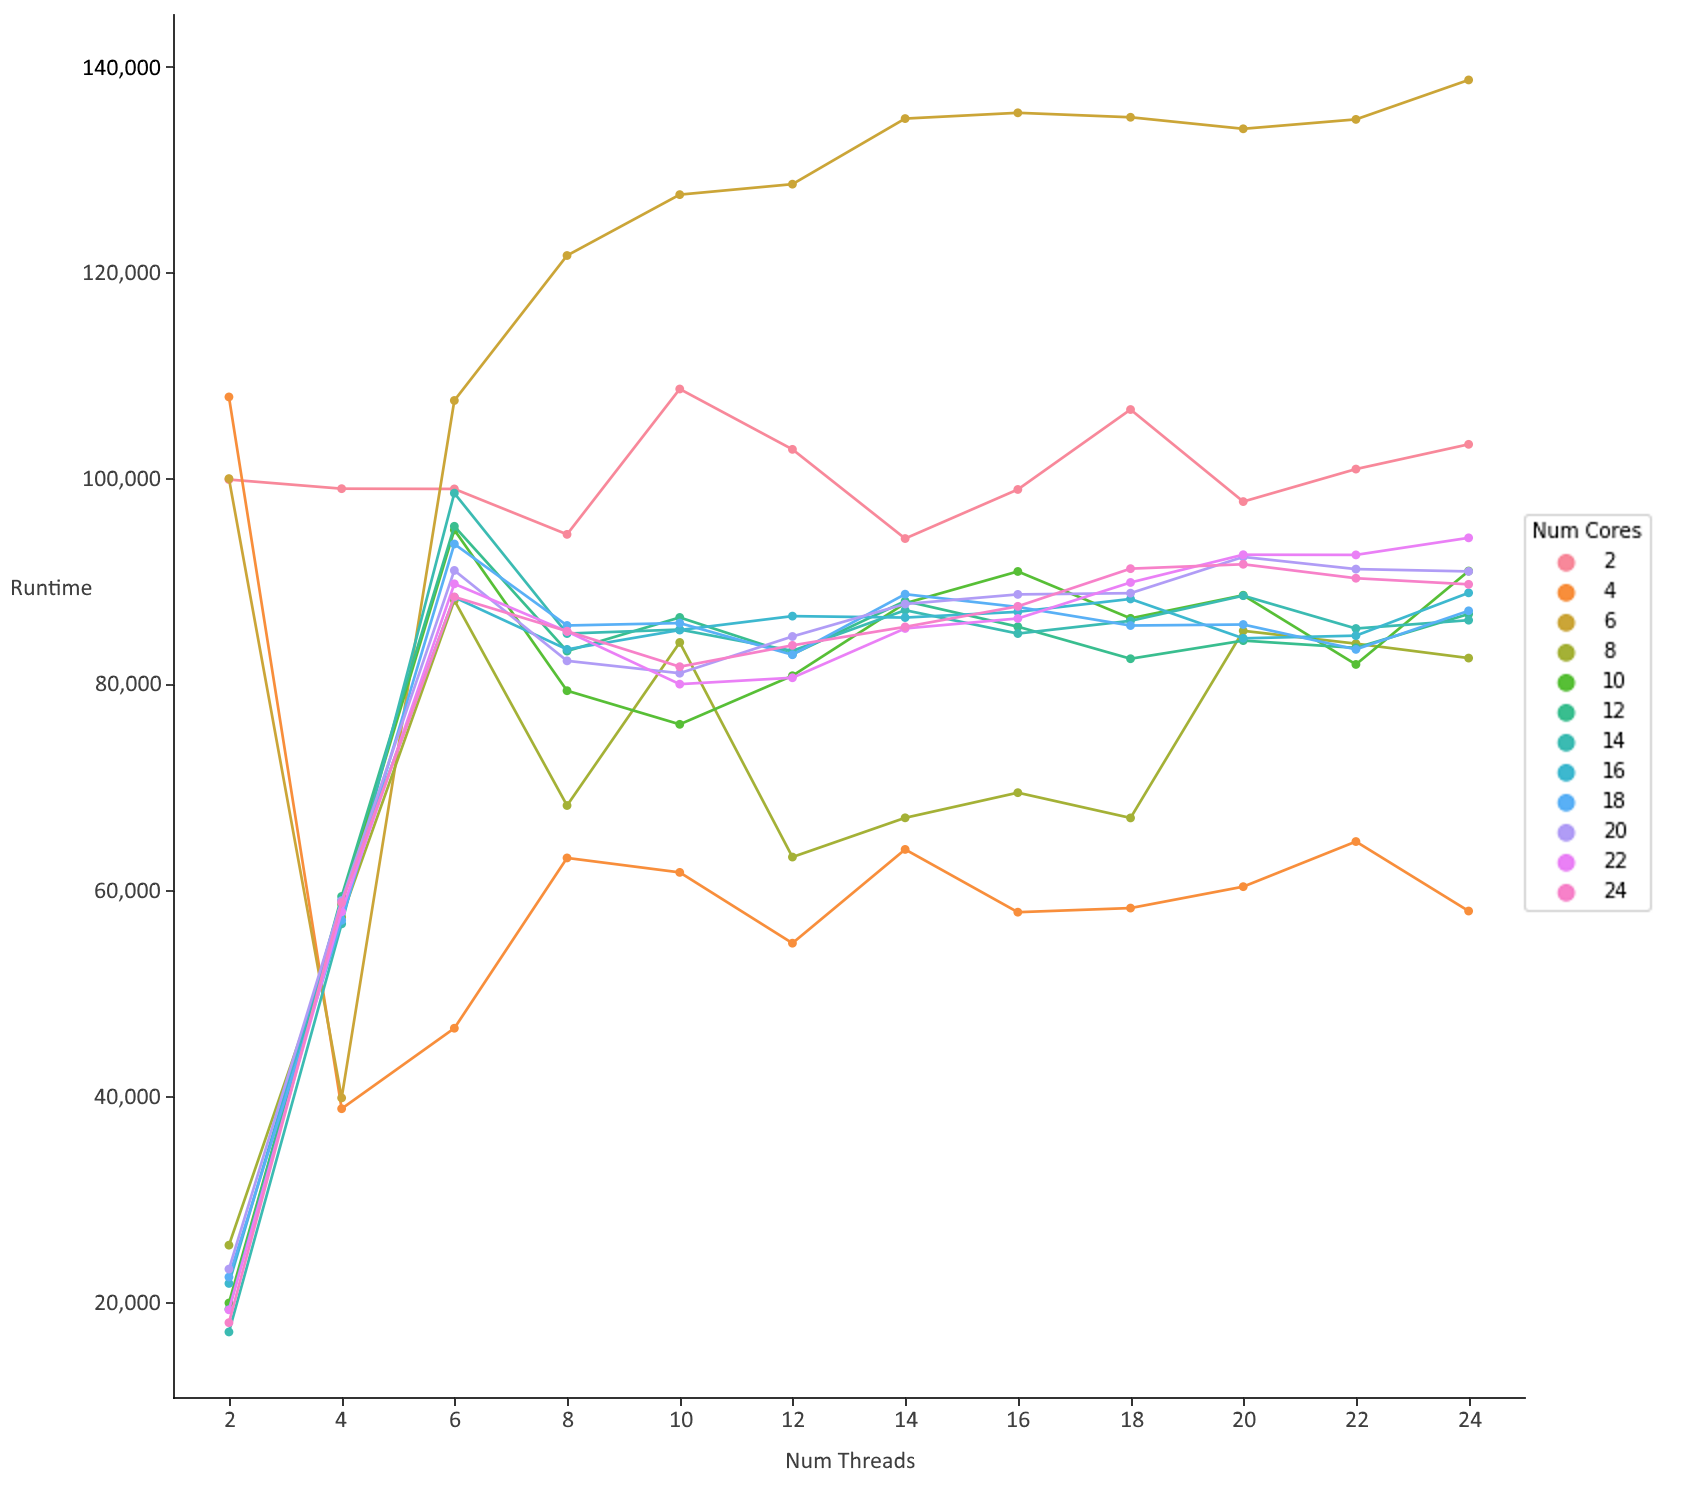
\includegraphics[width=1\textwidth]{graphics/optimal_threads_1.png}
    \caption{In this experiment, we provided the program with up to N CPU cores, and used up to N threads. Each number of threads was evaluated with each number of CPU cores in steps of 2. CPU core numbers from 1-12 are real cores, and 13-24 are hyperthreads.}
    \label{fig:optimal_threads_1}
\end{figure}



As figure \ref{fig:optimal_threads_1} shows, in the case where we utilise two cores (the pink line,) increasing the number of threads above two if anything degrades performance. This is as expected. Moving up to the case with four cores (the orange line,) we see a similar story, going above four threads degrades performance. However, for six cores (the yellow line,) we see something different. Using six threads results in drastically degraded performance. In general, we can see using six threads or more always hurts performance. This might still be expected, but we see that performance doesn't vary much above six threads regardless of how many cores are provided. We also see that using two workers with as many cores as possible is the optimal solution. Both of these facts are inconsistent with what we expect to see.

These results were produced quickly, using no repeats, as an initial investigation. So at first, we reasoned that this could be the result of cold cache issues, resulting in these strange runtimes. We reproduced the same experiment, using ten consecutive repeats. This produced the following graph in figure \ref{fig:optimal_threads_1_(repeats)}:



\begin{figure}[H]
    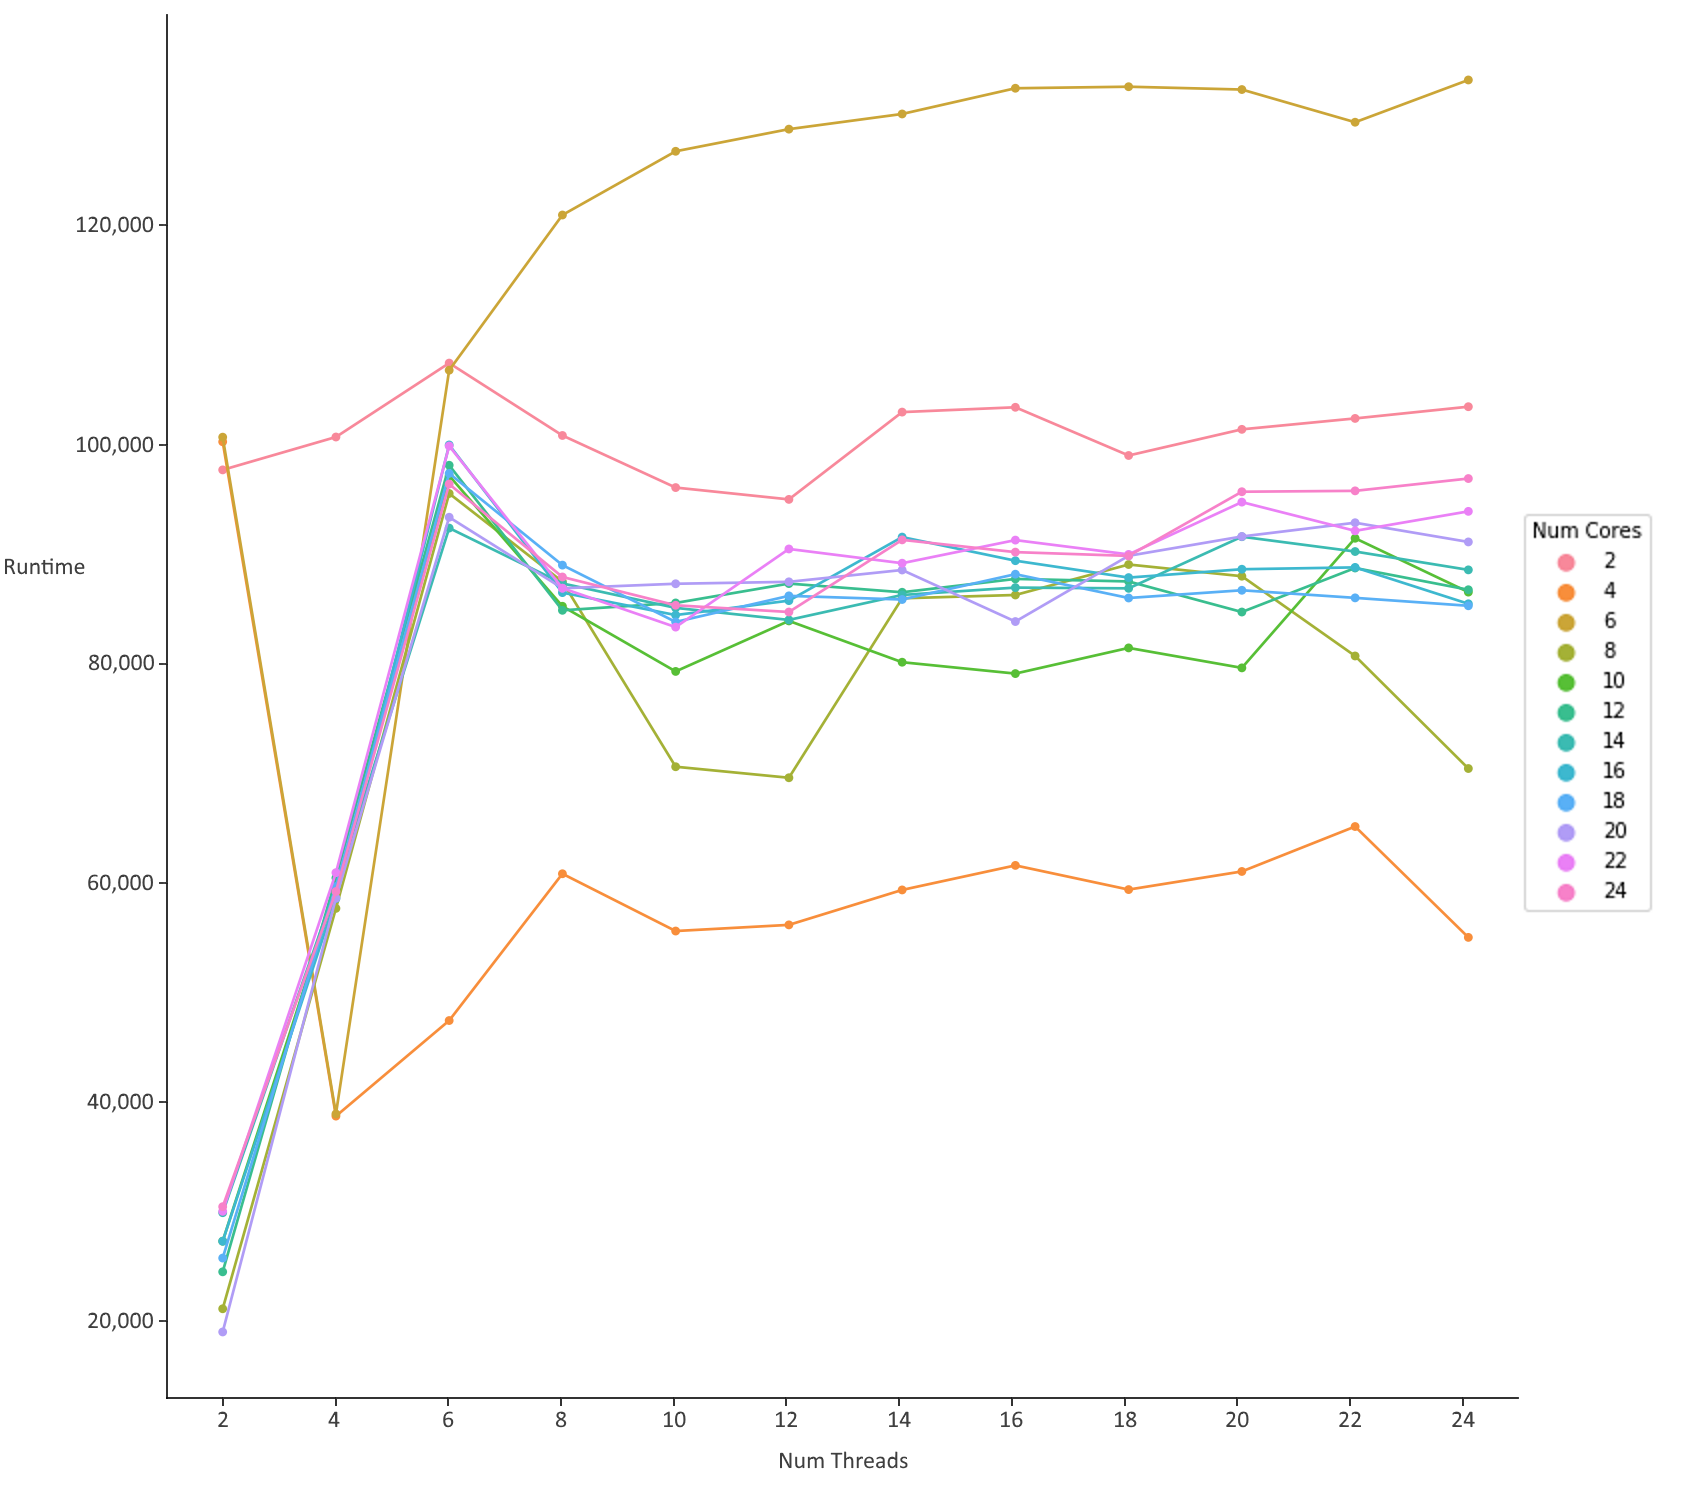
\includegraphics[width=1\textwidth]{graphics/optimal_threads_1_(repeats).png}
    \caption{As the previous experiment, only averaging the results over 10 repeated runs.}
    \label{fig:optimal_threads_1_(repeats)}
\end{figure}



Again, a similar story to the previous graph, with similar unexpected features. This rules out cache issues. 

After further diagnosis, we discovered some other strange behaviour. Running the computation with one thread resulted in times of ~500ms, and with two threads we saw ~20,000ms. Not what we would expect at all! Even stranger, when using multiple threads pinned to the same CPU we again saw runtimes in the region of ~500ms. 

Narrowing it down further, we changed the workload function from sqrt(rand()) to sin(rand()). This produced similar behaviour, so either the sqrt() and the sin() functions have the same issue, or the problem is the rand() function. The most likely culprit seemed to be the rand() function, so another method of preventing compiler optimisation was needed. This time, we tried using inline assembly code to provide the workload, so we can know exactly what is going on. An example of this is given in figure \ref{fig:asm_kernel} in appendix \ref{appendix:code_snippets}. But this still required a function wrapper, and preallocated memory.

It was after this that we discovered the volatile keyword. Quoting from the C++ Standard (7.1.5.1) \cite{cpp_standard}:

"Volatile is a hint to the implementation to avoid aggressive optimisation involving the object because the value of the object might be changed by means undetectable by an implementation."

Declaring the entire workload function as volatile successfully prevented the compiler from optimising it out, and solved our problem.

Upon further diagnosis, we found that the rand() function is not thread safe! This is consistent with the observed behaviour, since just one thread finished much faster, and many threads pinned to one core similarly fast. This was because, with all the threads running on the same core, they would never be running simultaneously, so calls to rand() would never interfere with each other. Using a non-thread safe function in this way is an easy to make, hard to diagnose error, and makes a good example of why parallel programming is hard.